%% *************************************************************************
%%
%% This is an RIT Space Exploration Standard defining guidelines for content
%% and formatting of project design documents.
%%
%% This document uses IEEEtran.cls, the official IEEE LaTeX class
%% for authors of the Institute of Electrical and Electronics Engineers
%% (IEEE) Transactions journals and conferences.
%%
%% *************************************************************************

%% *************************************************************************
% LaTeX REFERENCES
% ----------------
%   Intro to LaTeX: http://www.rpi.edu/dept/arc/docs/latex/latex-intro.pdf
%   Comprehensive LaTeX symbol list: http://tug.ctan.org/info/symbols/comprehensive/symbols-a4.pdf
%% *************************************************************************

% tell \LaTeX what kind of formatting to use
\documentclass[conference]{IEEEtran} % http://www.ctan.org/pkg/ieeetran
% enable placeholder text generator
\usepackage{blindtext}
% enable toolbox for embedding figures and pictures
\usepackage{graphicx}
% enable package for adding a list of variables and constants at the beginning, aka "nomenclature"
\usepackage{nomencl}
% enable package for easily formatting units
\usepackage{siunitx}
% enable package for cross-referencing figures, sections, references etc.
% how to use hyperref: http://www2.washjeff.edu/users/rhigginbottom/latex/resources/lecture09.pdf
\usepackage{hyperref}
% change text encoding to make it more crisp
\usepackage[T1]{fontenc}
% enable conditionals for help text
\usepackage{etoolbox}

% initialize nomenclature package
\makenomenclature{}

% set title. choose something as descriptive and precise as possible. Descriptive > sounding cool. remember this!
\title{High Level Exploration of Potential Space Mission Concepts}


\author{
  % List the authors of the design document. The Champion should go first.
  % The \$~\$ markers tell \LaTeX{} to treat the text inside to be treated as a math expression. This way you can use operators like \textcaret{} to place characters as superscripts.
  % Some \LaTeX{} templates handle the author block in different ways. For example, the \href{http://www.worldscientific.com/worldscinet/jai}{Journal of Astronomical Instrumentation} requires the authors' addresses and emails to be included as well.
  % The \textbackslash{}thanks command puts the contents inside those brackets in a footnote at the bottom of the first page. Technically speaking, \textbackslash{}thanks is just a specially formatted footnote.
  % IEEE also has a ``long form'' author block for many authors. Check here for more information:
  % \url{https://tex.stackexchange.com/questions/156523/multiple-authors-with-common-affiliations-in-ieeetran-conference-template}
  % Read here for a more advanced options to modifying footnotes in the author block:  \url{http://tex.stackexchange.com/questions/826/symbols-instead-of-numbers-as-footnote-markers}
  %   Here, we use the IEEE long-form author block.
  \IEEEauthorblockN{% This block is for author Names.
    T.J.~Tarazevits\IEEEauthorrefmark{1},
    Eric Gerstner\IEEEauthorrefmark{2},
  }
  \IEEEauthorblockA{% This block is for the author Afficliations, aka department and university
    RIT Space Exploration, Rochester Institute of Technology \\ %\\ starts a new line
    Rochester, N.Y. \\
    Email:
    \IEEEauthorrefmark{1}tjt3085@rit.edu,
    \IEEEauthorrefmark{2}egg2711@rit.edu,
  }
  %%   Below, we use the short-form author block and basically hack it to suit our needs.
  % Philip~Linden$^{*\dagger}$%
  %   \thanks{$^{*}$Project Champion}%
  %   \thanks{$^{\dagger}$BS/MEng '17, Mechanical Engineering},
  % Austin~Bodzas$^{\ddagger}$%
  %   \thanks{$^{\ddagger}$BS '19, Computer Science},
  % Drew~Walters$^{\S}$%
  %   \thanks{$^{\S}$BS '18, Mechanical Engineering Technology},
  % T.J.~Tarazevits$^{**}$%
  %   \thanks{$^{**}$BS '19, Game Design \& Development}%

  %%   If there are many authors, consider using symbolic, numeric (aka arabic),  alphabet footnotes or a combination thereof.
  %% the recommended order for symbolic footnotes is
  %%   (1) asterisk        *   *
  %%   (2) dagger          †   \dagger
  %%   (3) double dagger   ‡   \ddagger
  %%   (4) section symbol  §   \S
  %%   et cetera. For higher counts, use 2x symbols (1)-(4) (i.e. (5) two asterisks **). Keep cycling through (1)-(4) using 3x, 4x, and so on.
  %%   Note that these symbol codes work in math mode and text mode.
  %%   There are ways to make LaTeX do this for you, but it is more advanced and not entirely necessary, especially for short author lists. Not worth the hassle, in my opinion.
}
% page header for pages other than cover page
\markboth{Space Mission Feasibility Study}%
{Tarazevits \MakeLowercase{\textit{et al.}}: RIT Space Exploration}

% Initial setup is over, start building the document itself
\begin{document}
\maketitle%
% correct bad hyphenation here, separated by spaces
\hyphenation{explor-ation}

\begin{abstract}
This proposal defines a semester long research project to evaluate space mission concepts on a technical basis.
The chosen mission objective and constraints will be evaluated for their feasibility and potential solutions and technical approximations will be described in the final report.
It is intended to build technical skills as well as produce polished technical content that SPEX can showcase.

      % The abstract is a brief summary of the design document. Typically it includes the purpose of the design document, key goals or objectives, and justifications.
      % Be sure not to confuse the abstract with the introduction.
      % It is easiest to write the abstract after the rest of the paper has been written.
      % That way you can choose key information from the sections that you've already completed and string them together in the abstract.
      % Consider the abstract to be your elevator pitch to anyone reading this design document.
      % What are they reading?
      % What is the goal?
      % Why is it worth my time?
      % The abstract is what will show up in Google results and other search engines, and what people will read when they are deciding what is worth their time and brain power.
\end{abstract}

\label{sec:nomenclature}
\newcommand{\nomunit}[1]{%
\renewcommand{\nomentryend}{\hspace*{\fill}#1}}
\renewcommand{\nompreamble}{
    % If you include mathematical expressions or express variables in the design document, list them with their corresponding definitions here as a list.
    % The two lines below make it look nice when defining units/values to constants.

    % Note that math terms and non-math terms are separated and alphabetized, regardless of the order in which they are defined. (Recall terms \$like this\$ are in the math environment)
    % Read more about advanced nomenclature formatting here:\\
    % \url{https://www.sharelatex.com/learn/Nomenclatures}
  }
\nomenclature{RIT}{Rochester Institute of Technology}
\nomenclature{SPEX}{RIT Space Exploration}
\nomenclature{PDD}{Project Design Document}
% Below are examples of using nomenclature for math symbols and constants or units
% \nomenclature{$\dot{m}$}{Mass flow rate
%   \nomunit{\,\si{\kilo\gram\per\second}}}
% \nomenclature{$c$}{Speed of light
%  \nomunit{\,\SI{2.9979e8}{\meter\per\second}}}
\printnomenclature{}


% HELPFUL HINT: If you get the warning ``Command terminated with space.'' when using a \command try placing ``%'' or ``{}'' immediately following the command.

% The sections included here are required. Additional sections and subsections may be added as necessary.
\section{Introduction}
\label{sec:introduction}
  % The introduction is a place to give background and context before diving into the subject matter.
  % Establish context for the work you are about to propose and the main ideas of the proposition itself.

\IEEEPARstart{I}{n} the spring of 2016, SPEX advisors conducted a Special Topics Course on Astrodynamics and Satellite Engineering.
One of the projects undertaken for this course was a high level mission feasibility study, wherein an objective was selected, and preliminary mission parameters were given to student teams.
Each team assumed the responsibility of exploring the physical and technical challenges for the mission, and proposing solutions and designs for accomplishing the objective.
This project would be a natural expansion upon that process, where student teams would be given new parameters and objectives and tasked with evaluating the feasibility and technical complexity of achieving those goals.
The missions explored do not need to conform to the cubesat standard or be restricted to what an undergraduate research team could afford to construct.

\section{Primary Objective}
\label{sec:primary-obj}
  % At the end of the day, whether the project ``succeeds'' or ``fails'' is judged against the objectives it sought to meet.
  % Note that results that contradict expectations/hypotheses are not failures if the scientific \& engineering methods are followed along the way.
  % Sometimes our expectations are wrong and that can be just as successful as getting data we thought we'd see.
  % What matters are what questions you intend to answer.
  % This is the main purpose or main goal the project hopes to achieve.

The goal is to engage students in the practice of astronautical engineering by presenting them with challenges encountered in the field and using applicable techniques and technology to solve problems.

Students will learn about the unique environmental conditions and practical engineering restrictions astronautical engineering presents, and become familar with the mathematical equations and physical properties that apply to that environment.
%\begin{figure}
%  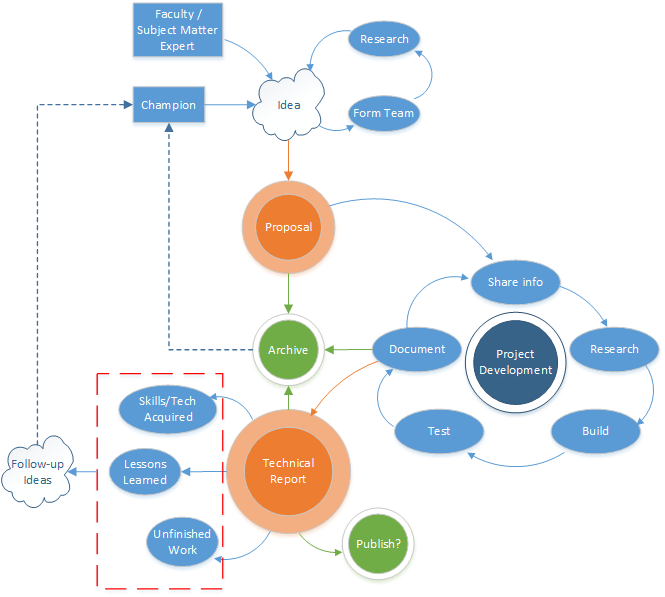
\includegraphics[width=\linewidth]{figs/project-life-cycle.png}
%  \caption{A PDD is the first piece of documentation to be archived in the project life cycle. Since the life cycle can be iterative, a new design document may also refer to one or more previous SPPs.}
%\label{fig:lifecycle}
%\end{figure}

% \section{Secondary Objectives}
% \label{sec:secondary-obj}
% Secondary Objectives are lower priority or bonus objectives that are significant but not the main focus of the project. This template does not have secondary objectives.

\section{Benefit to SPEX}
\label{sec:benefit}
% One of the core values of SPEX is to provide opportunities for academic and professional growth for its members,
% and to challenge them with interesting projects.
% In this section, explain how the project would benefit SPEX members as students,
% space enthusiasts, and young professionals.

This project will have several key benefits to SPEX in the near and long-term.
This project will encourage an astronautical engineering mindset among SPEX members, and will drive technical excellence for all of SPEX's projects.

% Below I have used subsections to identify key ideas in this section. These particular subsections are not required as part of the SPEX Standard, but serve as an example of using subsections in a text.

\subsection{Technical Skills}
\label{subsec:mindset}
Firstly, this project requires members seek out practical engineering knowledge to solve challenges.
Members will learn the mathematical process for calculating various mission and vehicle parameters.
Also, systems-level knowledge will be required to ensure each sub-system can fit within the mass and volume bounds set by the project.
Applying these skills is incredibly valuable, and will make members more attrative to employers, as well as build their technical competency when working on other SPEX projects.

\subsection{Published Content}
\label{subsec:traceability}
Similarly, the end goal of this project is a highly polished technical document that can be shared internally within SPEX, and self-published externally for the RIT or broader aerospace community to read.
This will build SPEX's legitimacy when compared to other school's aerospace programs, and act as a first-class representation of SPEX's technical competency that can be shared with employers and potential sponsors.

\subsection{Future Project Feasibility}
\label{subsec:plug-n-play}
  % Note below that LaTeX uses weird formatting when it comes to quotation marks.
  % The style below is correct to display forward quotes `` at the start of the phrase and backquotes '' at the end.
As each finished study is intended to be a high level overview of potential challenges and solutions, they will provide a launch pad for other studies, reports, and projects.
For example, a high level design for a probe landing system as part of a general lander mission, could be expanded upon in its own project, either as an in-depth report, or prototype engineering test article.
Solutions investigated during the course of this project could be applied to other SPEX projects as well.
Alternatively, problems and risk areas addressed in these studies will inform members working on future projects, and provide valuable experience.
\section{Implementation}
\label{sec:implementation}
  % What path do you anticipate the project to take?
The project will begin with selecting a primary mission objective, and establishing constraints, e.g. vehicle parameters, total cost, etc.
This process could involve SPEX advisor input, finding other RIT faculty with existing mission concepts, or identifying areas of interest defined by NASA, ESA, etc.

The process will involve research, using RIT academic resources and other externally available media, to identify key challenge areas and potential solutions.
Then constraints and solutions will be calculated mathetically. For example, given the requirement to transmit an image of given dimensions and total size, what are the radio requirements to trasmit that data in an expedient manner?
This solutions will be checked by other members within the team, and also presented to SPEX advisors and other advising faculty.
Then the teams will iterate, incorporating feedback and suggestions to eventually arrive at ideal designs.

At the end of the project (or end of semester, whichever comes first), the team writes the final report, showcasing the potential solutions to the mission objective, as well as the overall feasibility of the mission with the given constraints.
Also, the mission may be a candidate for the AIAA Space conference, and an abstract could be submitted in early December.

\subsection{Deliverables}
\label{subsec:deliverables}
  % When all is said and done, what will you have to show for it?
  % Examples: Hardware, software, poster, ImagineRIT demo, presentations, technical papers...
The primary deliverable will be a polished report that can be published if SPEX chooses.
Incorporated within the document will be clear definitions of the mission objective, external constraints, and any assumptions made by the team.
Mathematical equations will be included as necessary, to showcase the mathematical foundations on which mission parameters were derived.
Charts, graphs, and other data visualizations are highly encouraged, especially when they showcase a range of potential solutions and indicate why the team chose certain parameters.
Sketches, CAD models, and other graphics will be included to aid the reader in visualizing the complete system and other novel solutions designed by the team.
\subsection{Milestones}
\label{subsec:milestones}
  % Be as detailed as you can, but it's okay if there are unknowns.
  % At the very least, specify how many semester you expect the project to take until it reaches completion.
If this project is conducted over a semester timeline, the team will need to expediently cover the required areas defined below.
\begin{itemize}
  \item Select mission objective and define constraints - no more than 2 weeks
  \item Research key technical areas - no more than 4 weeks
  \item Develop initial solution
  \item Iterate on solution and technical analysis
  \item Choose areas of importance to delve more deeply for technical insight
  \item Iterate on final deliverable
  \item Present finished study to SPEX adivsors and general group
\end{itemize}

The latter objectives can be handled in a variety of development techniques, e.g. waterfall, scrum, agile, etc
\section{Externalities}
  % Things not directly related to the work or outcomes, but related to the project as a whole.
\subsection{Prerequisite Skills}
  % Which skills do team members need to have before work can start (not including skills that will be learned ``on the job'')?
While some of the mathematics involved only requires basic algebra and trigonometry, members are recommended to have calculus experience.
Existing astronatical engineering experience is obviously preferred, but the goal of this project is to build that skillset, so it is not required.jk
The challenges and equations this project requires are unlikely to be covered in most courses at RIT, especially in lower year levels, so members should expect to deal with a lot of never before seen material.

\subsection{Funding Requirements}
  % Estimate costs that would be needed to meet objectives.
This project is unlikely to require direct funding. All work will consist of research, calculations, and producing a report using free or easily accessible tools.

\subsection{Faculty Support}
  % Identify faculty that will be involved (or would need to be involved) to meet objectives.
  % Note that if a professor is the Principal Investigator (P.I.) for a project, there still needs to be a student as the SPEX Project Champion.
Faculty support is highly recommended for teams pursing this project.
Teams should look for potential mission ideas from RIT faculty, across colleges and departments.
SPEX advisors would play a key guidng role for the team, acting as de facto reviewers during the iterative phase of the process.
\subsection{Long-Term Vision}
\label{sec:vision}
As SPEX successfuly completes these feasibility studies, they will naturally provide starting points for continuation studies and other projects.
AIAA Space is a potential publishing opportunity, offering a platform that accepts a variety of papers on potential mission solutions.
If accepted, students from the team could apply for RIT travel grants to attend and present the paper to the wider aerospace community.

Another long-term goal would be to continue the development cycle, converting a feasibility study into an actual mission plan, and finally into an actual space mission.
However, the scope of such an implementation is outside of the present and near-term ability of SPEX.
\section*{Acknowledgements}
The authors would like to thank Dr. Dorin Patru for the initial mission feasibility study this project is based off of, as well as Dr. Mihail Barbosu and Dr. Jennifer Connelly, the other SPEX advisors who taught the Special Topics Course on Astrodynamics and Satellite Engineering.

%\onecolumn
%\appendices{}
%\section{Project Life Cycle}
%\begin{figure}[h]
%\end{figure}  \centering
%  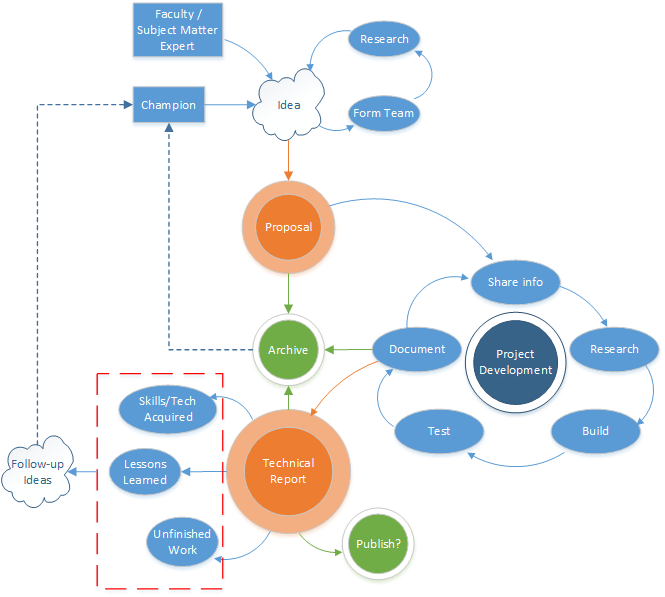
\includegraphics[]{figs/project-life-cycle.png}
%  \caption{Enlarged version of the diagram in \autoref{fig:lifecycle}.}
%\end{figure}

\end{document}
